\documentclass[11pt, letterpaper]{article}

\usepackage[margin=1in]{geometry}
\usepackage{graphicx}
\usepackage{booktabs}
\usepackage{enumitem}
\usepackage{tikz}
\usepackage{xcolor}
\usepackage{hyperref}
\usepackage{fancyhdr}
\usepackage{tabularx}
\usepackage{amsmath}

\usetikzlibrary{shapes.geometric, arrows.meta, positioning, fit, backgrounds, calc}

% Colors
\definecolor{primary}{HTML}{2563EB}
\definecolor{secondary}{HTML}{7C3AED}
\definecolor{accent}{HTML}{059669}
\definecolor{warm}{HTML}{D97706}
\definecolor{lightbg}{HTML}{F1F5F9}
\definecolor{darktext}{HTML}{1E293B}

\hypersetup{
    colorlinks=true,
    linkcolor=primary,
    urlcolor=primary,
    citecolor=secondary
}

\pagestyle{fancy}
\fancyhf{}
\rhead{Capstone II --- Memory Architecture}
\lhead{Conversation-to-Calendar AI}
\rfoot{Page \thepage}

\title{\textbf{LLM Memory Architectures}\\[0.3em]
\large Approaches for Persistent State in the\\Conversation-to-Calendar AI Pipeline}
\author{Capstone Project II}
\date{February 2026}

\begin{document}
\maketitle
\thispagestyle{fancy}

% ============================================================
\section{Overview}

The calendar AI pipeline currently operates statelessly---each conversation transcript
is processed independently with no memory of prior interactions. Adding persistent memory
enables the system to learn user preferences, remember relationships, and make increasingly
accurate scheduling decisions over time.

This document outlines three architectural approaches used by production LLM memory systems,
analyzes their tradeoffs, and identifies the best fit for our single-user demo pipeline.

\subsection{The Universal Memory Lifecycle}

Regardless of architecture, every production memory system follows the same logical lifecycle:

\begin{enumerate}[leftmargin=2em]
    \item \textbf{Extract} --- Identify candidate facts from the conversation
    \item \textbf{Retrieve} --- Search existing memory for similar/related entries
    \item \textbf{Decide} --- Determine action: \textsc{add}, \textsc{update}, \textsc{delete}, or \textsc{noop}
    \item \textbf{Store} --- Persist the decision to the memory backend
    \item \textbf{Inject} --- Load relevant memories into future prompts
\end{enumerate}

\noindent The key differentiator between approaches is \emph{who} performs steps 1--3
and \emph{when} they occur relative to the main task.

% ============================================================
\section{Approach A: Dual-Call Pipeline}
\label{sec:dual-call}

\subsection{Description}

A \textbf{separate, dedicated LLM call} extracts memories after the main task completes.
A second LLM call compares extracted facts against existing memories (retrieved via
similarity search) and decides the appropriate action for each.

This is the pattern used by \textbf{Mem0} (37k+ GitHub stars) and forms the basis
of most RAG-augmented memory systems.

\subsection{Architecture}

\begin{center}
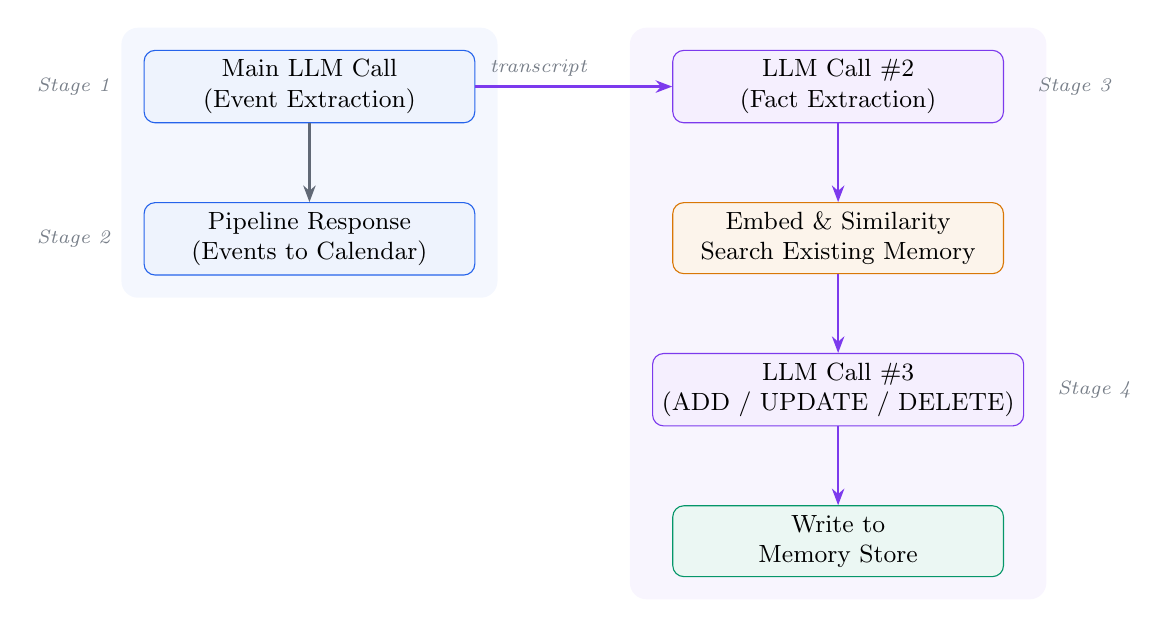
\begin{tikzpicture}[
    node distance=1.0cm and 2.0cm,
    box/.style={rectangle, draw=#1, fill=#1!8, rounded corners=4pt,
                minimum width=4.2cm, minimum height=0.9cm, align=center,
                font=\small},
    arrow/.style={-{Stealth[length=6pt]}, thick, color=darktext!70},
    label/.style={font=\scriptsize\itshape, text=darktext!60}
]

% Main pipeline (left)
\node[box=primary] (task) {Main LLM Call\\(Event Extraction)};
\node[box=primary, below=of task] (response) {Pipeline Response\\(Events to Calendar)};

% Memory pipeline (right)
\node[box=secondary, right=2.5cm of task] (extract) {LLM Call \#2\\(Fact Extraction)};
\node[box=warm, below=of extract] (search) {Embed \& Similarity\\Search Existing Memory};
\node[box=secondary, below=of search] (decide) {LLM Call \#3\\(ADD / UPDATE / DELETE)};
\node[box=accent, below=of decide] (store) {Write to\\Memory Store};

% Arrows
\draw[arrow] (task) -- (response);
\draw[arrow, color=secondary] (task.east) -- ++(0.8,0) |- (extract.west)
    node[label, pos=0.25, above] {transcript};
\draw[arrow, color=secondary] (extract) -- (search);
\draw[arrow, color=secondary] (search) -- (decide);
\draw[arrow, color=secondary] (decide) -- (store);

% Labels
\node[label, left=0.3cm of task] {Stage 1};
\node[label, left=0.3cm of response] {Stage 2};
\node[label, right=0.3cm of extract] {Stage 3};
\node[label, right=0.3cm of decide] {Stage 4};

% Grouping
\begin{scope}[on background layer]
    \node[fit=(task)(response), fill=primary!5, rounded corners=6pt,
          inner sep=8pt, label={[font=\small\bfseries, text=primary]above:Task Pipeline}] {};
    \node[fit=(extract)(search)(decide)(store), fill=secondary!5, rounded corners=6pt,
          inner sep=8pt, label={[font=\small\bfseries, text=secondary]above:Memory Pipeline}] {};
\end{scope}

\end{tikzpicture}
\end{center}

\subsection{How the Decision Works}

The action-decision LLM receives a structured prompt:

\begin{quote}
\small
\texttt{Existing Memory:}\\
\texttt{~~[id: abc123] "Alice prefers morning meetings"}\\
\texttt{~~[id: def456] "Bob is Alice's manager"}\\[0.5em]
\texttt{New Extracted Facts:}\\
\texttt{~~"Alice now prefers meetings before 10am"}\\[0.5em]
\texttt{For each fact, output: \{ADD | UPDATE | DELETE | NOOP\}}
\end{quote}

\noindent The LLM outputs structured JSON with the action, target memory ID (if updating/deleting),
and the new or merged text.

\subsection{Key Characteristics}

\begin{itemize}[leftmargin=2em]
    \item \textbf{Model:} Can use a cheap/fast model for extraction (Mem0 defaults to
          \texttt{gpt-4.1-nano}; we would use Gemini Flash)
    \item \textbf{Separation:} Main task quality is completely unaffected by memory overhead
    \item \textbf{Deduplication:} Similarity search retrieves candidates; LLM makes the
          semantic decision (supplementary vs.\ contradictory)
    \item \textbf{Cost:} 2 additional LLM calls per pipeline run + embedding calls
    \item \textbf{Latency:} Sequential post-processing; can be made async
\end{itemize}

\subsection{Tradeoffs}

\begin{table}[h]
\centering
\begin{tabularx}{\textwidth}{lXX}
\toprule
\textbf{Dimension} & \textbf{Advantage} & \textbf{Disadvantage} \\
\midrule
Separation of concerns & Memory logic fully decoupled from task & Extraction LLM may miss conversational nuance \\
Cost & Can use cheapest model for memory & 2+ extra LLM calls per interaction \\
Tunability & Memory prompts tuned independently & More prompts to maintain \\
Complexity & Clean pipeline stages & Pipeline orchestration overhead \\
Audit trail & Full CRUD history in storage & More storage writes \\
\bottomrule
\end{tabularx}
\end{table}

\subsection{Production Examples}

\begin{description}[leftmargin=2em, style=nextline]
    \item[Mem0] Open-source memory layer (37k+ stars). Uses vector DB (Qdrant) +
        optional graph DB (Neo4j). MD5 hashing for exact-duplicate detection.
        \texttt{ThreadPoolExecutor} writes to vector and graph stores in parallel.
    \item[LangMem (background mode)] Post-conversation reflection via
        \texttt{create\_memory\_store\_manager}. Full conversation analysis with
        schema-enforced (Pydantic) structured output.
\end{description}

% ============================================================
\section{Approach B: Self-Editing Agent}
\label{sec:self-editing}

\subsection{Description}

The \textbf{same LLM} that handles the main task also manages memory via \textbf{tool calls}
during its reasoning loop. The model decides what to remember as part of generating its
response---no separate extraction step.

This is the pattern used by \textbf{MemGPT/Letta} and \textbf{ChatGPT}.

\subsection{Architecture}

\begin{center}
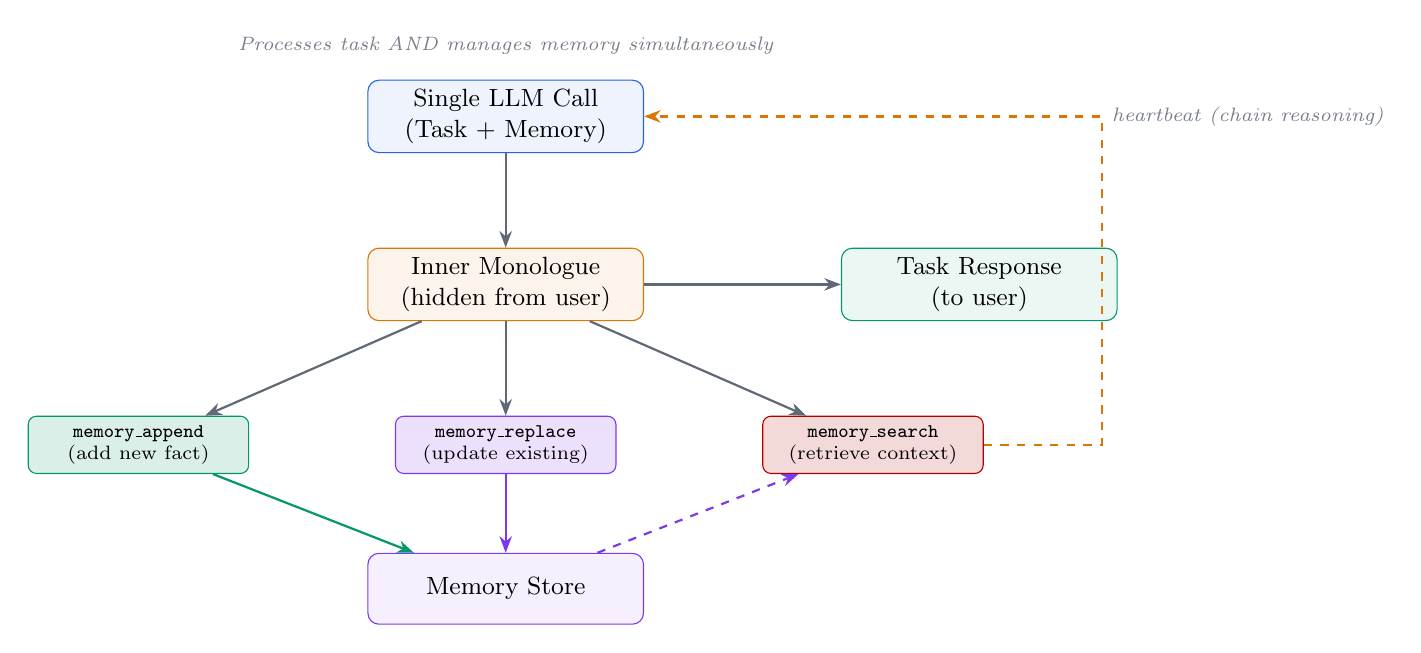
\begin{tikzpicture}[
    node distance=0.8cm and 1.5cm,
    box/.style={rectangle, draw=#1, fill=#1!8, rounded corners=4pt,
                minimum width=3.5cm, minimum height=0.9cm, align=center,
                font=\small},
    tool/.style={rectangle, draw=#1, fill=#1!15, rounded corners=3pt,
                 minimum width=2.8cm, minimum height=0.7cm, align=center,
                 font=\scriptsize},
    arrow/.style={-{Stealth[length=6pt]}, thick, color=darktext!70},
    label/.style={font=\scriptsize\itshape, text=darktext!60}
]

% Central agent
\node[box=primary] (agent) {Single LLM Call\\(Task + Memory)};
\node[label, above=0.2cm of agent] {Processes task AND manages memory simultaneously};

% Inner monologue
\node[box=warm, below=1.2cm of agent] (inner) {Inner Monologue\\(hidden from user)};

% Tool calls (fan out)
\node[tool=accent, below left=1.2cm and 1.5cm of inner] (t1) {\texttt{memory\_append}\\(add new fact)};
\node[tool=secondary, below=1.2cm of inner] (t2) {\texttt{memory\_replace}\\(update existing)};
\node[tool=red!70!black, below right=1.2cm and 1.5cm of inner] (t3) {\texttt{memory\_search}\\(retrieve context)};

% Response
\node[box=accent, right=2.5cm of inner] (resp) {Task Response\\(to user)};

% Memory store
\node[box=secondary, below=1.0cm of t2] (store) {Memory Store};

% Arrows
\draw[arrow] (agent) -- (inner);
\draw[arrow] (inner) -- (t1);
\draw[arrow] (inner) -- (t2);
\draw[arrow] (inner) -- (t3);
\draw[arrow] (inner) -- (resp);
\draw[arrow, color=accent] (t1) -- (store);
\draw[arrow, color=secondary] (t2) -- (store);
\draw[arrow, color=secondary, dashed] (store) -- (t3);

% Heartbeat loop
\draw[arrow, color=warm, dashed] (t3.east) -- ++(1.5,0) |- (agent.east)
    node[label, pos=0.5, right] {heartbeat (chain reasoning)};

\end{tikzpicture}
\end{center}

\subsection{How It Works}

The LLM's context window contains the current memory state directly. During reasoning,
the model generates an \emph{inner monologue} (not shown to the user), then issues
tool calls:

\begin{quote}
\small
\texttt{Inner thought: "The user mentioned they prefer afternoons}\\
\texttt{now. I should update my memory."}\\[0.3em]
\texttt{Tool call: memory\_replace(}\\
\texttt{~~old="Alice prefers morning meetings",}\\
\texttt{~~new="Alice prefers afternoon meetings")}
\end{quote}

\noindent MemGPT uses a \texttt{request\_heartbeat} flag that returns control to the LLM
after a tool call, enabling multi-step memory operations (search $\rightarrow$ read $\rightarrow$ update)
in a single interaction.

\subsection{Memory Tiers (MemGPT)}

\begin{table}[h]
\centering
\begin{tabularx}{\textwidth}{llX}
\toprule
\textbf{Tier} & \textbf{Analogy} & \textbf{Properties} \\
\midrule
Core Memory & RAM & In-context, read-write, bounded ($\sim$2000 tokens). Persona + Human blocks. \\
Recall Storage & Page file & Full conversation logs, searchable, out-of-context. \\
Archival Storage & Disk & Unbounded, vector-searchable, long-term facts. \\
\bottomrule
\end{tabularx}
\end{table}

\subsection{Tradeoffs}

\begin{table}[h]
\centering
\begin{tabularx}{\textwidth}{lXX}
\toprule
\textbf{Dimension} & \textbf{Advantage} & \textbf{Disadvantage} \\
\midrule
Cost & Single LLM call & May need heartbeat chains (multiple rounds) \\
Latency & Memory ops during response generation & Increased per-response latency \\
Context & Full conversational nuance available & Cognitive load: task + memory simultaneously \\
Simplicity & No separate pipeline & Agent may ``forget to remember'' under load \\
Autonomy & Agent reasons about \emph{why} to store & Harder to tune memory independently \\
\bottomrule
\end{tabularx}
\end{table}

\subsection{Production Examples}

\begin{description}[leftmargin=2em, style=nextline]
    \item[MemGPT / Letta] Open-source OS-inspired memory. Six memory tools
        (\texttt{core\_memory\_append}, \texttt{core\_memory\_replace},
        \texttt{archival\_memory\_insert}, \texttt{archival\_memory\_search},
        \texttt{conversation\_search}, \texttt{send\_message}).
        Memory pressure triggers automatic eviction when context reaches $\sim$70\%.
    \item[ChatGPT] Uses a \texttt{bio} tool. Memories stored as short, timestamped
        sentences. Triggers: explicit (``remember that\ldots'') or implicit
        (model detects noteworthy info and user confirms through conversation).
\end{description}

% ============================================================
\section{Approach C: Hybrid (Hot + Background)}
\label{sec:hybrid}

\subsection{Description}

Combines both approaches: a \textbf{hot path} captures memories during the conversation
(like Approach B), while a \textbf{background path} runs a deeper analysis after the
conversation ends (like Approach A). This maximizes both immediacy and recall.

This is the pattern supported by \textbf{LangMem / LangGraph}.

\subsection{Architecture}

\begin{center}
\begin{tikzpicture}[
    node distance=0.8cm and 1.8cm,
    box/.style={rectangle, draw=#1, fill=#1!8, rounded corners=4pt,
                minimum width=3.8cm, minimum height=0.9cm, align=center,
                font=\small},
    arrow/.style={-{Stealth[length=6pt]}, thick, color=darktext!70},
    label/.style={font=\scriptsize\itshape, text=darktext!60}
]

% Input
\node[box=darktext] (input) {User Conversation};

% Fork
\node[box=primary, below left=1.5cm and 1.5cm of input] (hot) {Hot Path\\(During Conversation)};
\node[box=secondary, below right=1.5cm and 1.5cm of input] (bg) {Background Path\\(After Conversation)};

% Hot path detail
\node[box=primary, below=0.8cm of hot] (hottools) {Agent Tool Calls\\(\texttt{manage\_memory})};

% Background path detail
\node[box=secondary, below=0.8cm of bg] (bgworker) {Async Memory Worker\\(Full Convo Analysis)};

% Shared store
\node[box=accent, below=1.5cm of input, yshift=-4.5cm] (store) {Shared Memory Store\\(LangGraph BaseStore)};

% Schema
\node[tool=warm, left=2.0cm of store] (collection) {Collection Mode\\(Multiple docs, CRUD)};
\node[tool=warm, right=2.0cm of store] (profile) {Profile Mode\\(Single doc, patches)};

% Arrows
\draw[arrow] (input) -| (hot);
\draw[arrow] (input) -| (bg);
\draw[arrow, color=primary] (hot) -- (hottools);
\draw[arrow, color=secondary] (bg) -- (bgworker);
\draw[arrow, color=primary] (hottools) -- (store)
    node[label, midway, left] {immediate};
\draw[arrow, color=secondary] (bgworker) -- (store)
    node[label, midway, right] {deferred};
\draw[arrow, dashed, color=warm] (store) -- (collection);
\draw[arrow, dashed, color=warm] (store) -- (profile);

\end{tikzpicture}
\end{center}

\subsection{Two Formation Paths}

\begin{description}[leftmargin=2em]
    \item[Hot Path (``Conscious'')] Agent calls \texttt{manage\_memory()} and
        \texttt{search\_memory()} tools during conversation. Immediate availability
        but limited to what the agent notices in real-time.
    \item[Background Path (``Subconscious'')] After conversation ends, a
        \texttt{create\_memory\_store\_manager} analyzes the full transcript.
        Higher recall---catches patterns the hot path missed. Uses \texttt{trustcall}
        for schema-validated extraction with parallel tool calling.
\end{description}

\subsection{Tradeoffs}

\begin{table}[h]
\centering
\begin{tabularx}{\textwidth}{lXX}
\toprule
\textbf{Dimension} & \textbf{Advantage} & \textbf{Disadvantage} \\
\midrule
Coverage & Maximum recall (two extraction passes) & Risk of duplicate processing \\
Latency & Hot path: immediate; background: zero user-facing & Background memories are stale until processed \\
Flexibility & Configurable: hot only, background only, or both & Most complex to configure and operate \\
Consistency & Schema-enforced structured memory (Pydantic) & Framework-dependent (LangGraph ecosystem) \\
\bottomrule
\end{tabularx}
\end{table}

% ============================================================
\section{Comparative Analysis}

\subsection{Decision Matrix}

\begin{table}[h]
\centering
\small
\begin{tabularx}{\textwidth}{lXXX}
\toprule
\textbf{Dimension} & \textbf{A: Dual-Call} & \textbf{B: Self-Editing} & \textbf{C: Hybrid} \\
\midrule
Who extracts & Dedicated LLM & Same LLM (tools) & Both \\
Extraction model & Cheap/fast model & Task model & Configurable \\
Decision method & LLM (2nd call) & Agent tool calls & LLM via \texttt{trustcall} \\
Conflict handling & LLM decides action & Agent replaces text & RemoveDoc + insert \\
Cost per run & 2+ extra LLM calls & 1 call (+ heartbeats) & 1--3 calls \\
Task interference & None & Cognitive load risk & Configurable \\
Audit trail & Full CRUD history & Agent-logged & Schema-enforced \\
\bottomrule
\end{tabularx}
\end{table}

\subsection{Key Architectural Insight}

Every production system uses an \textbf{LLM to make the ADD/UPDATE/DELETE decision}---not
just similarity thresholds. Cosine similarity retrieves candidate matches, but only an
LLM can distinguish:

\begin{itemize}[leftmargin=2em]
    \item \textbf{Supplementary:} ``prefers mornings'' + ``likes 9am slots''
          $\rightarrow$ \textsc{update} (merge)
    \item \textbf{Contradictory:} ``prefers mornings'' + ``switched to afternoons''
          $\rightarrow$ \textsc{update} (replace)
    \item \textbf{Redundant:} ``prefers mornings'' + ``likes morning meetings''
          $\rightarrow$ \textsc{noop}
\end{itemize}

% ============================================================
\section{Recommendation}

For our single-user demo pipeline, \textbf{Approach A (Dual-Call)} is the best fit:

\begin{enumerate}[leftmargin=2em]
    \item \textbf{Matches existing architecture.} The pipeline already injects calendar
          context into the system prompt. Memory context follows the same pattern---a
          second injection section alongside ``Your Calendar.''
    \item \textbf{Clean separation.} Event extraction quality (the core product) remains
          unaffected by memory overhead. Memory prompts can be tuned independently.
    \item \textbf{Gemini Flash is cheap.} At \$0.15/1M input tokens, two extra Flash calls
          per pipeline run are negligible. No need for a separate nano model.
    \item \textbf{No new infrastructure.} SQLite (stdlib) for storage. No vector DB, no
          embeddings---at single-user scale ($<$100 memories), full injection outperforms
          semantic retrieval.
    \item \textbf{Demo-friendly.} The memory extraction step produces visible, loggable
          output showing the AI ``learning''---a compelling demo artifact.
\end{enumerate}

\noindent The simplified flow for our pipeline:

\begin{center}
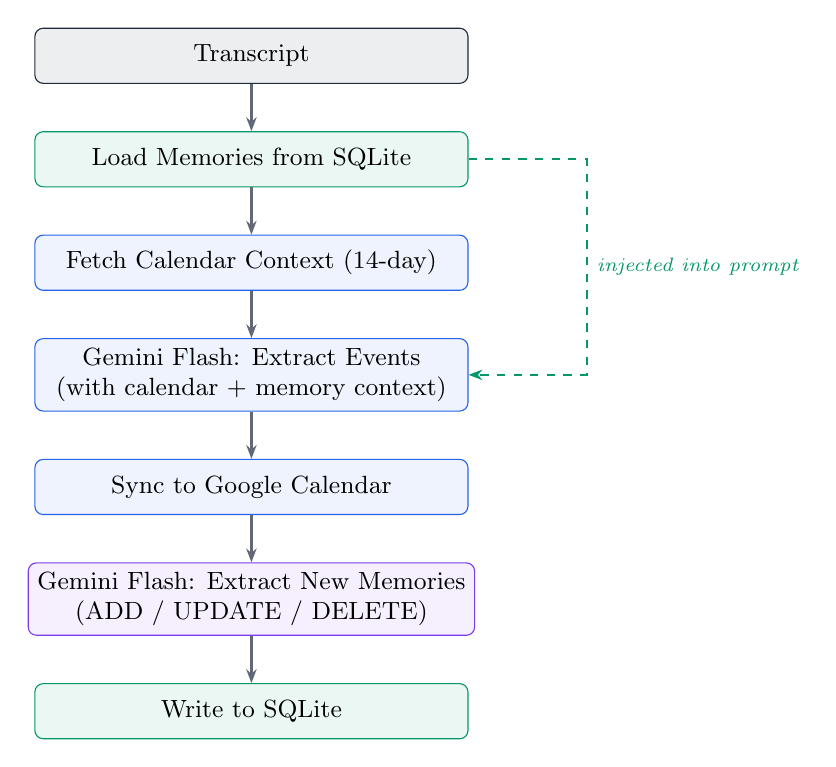
\begin{tikzpicture}[
    node distance=0.6cm,
    box/.style={rectangle, draw=#1, fill=#1!8, rounded corners=3pt,
                minimum width=5.5cm, minimum height=0.7cm, align=center,
                font=\small},
    arrow/.style={-{Stealth[length=5pt]}, thick, color=darktext!70}
]

\node[box=darktext] (t) {Transcript};
\node[box=accent, below=of t] (mem) {Load Memories from SQLite};
\node[box=primary, below=of mem] (cal) {Fetch Calendar Context (14-day)};
\node[box=primary, below=of cal] (llm) {Gemini Flash: Extract Events\\(with calendar + memory context)};
\node[box=primary, below=of llm] (sync) {Sync to Google Calendar};
\node[box=secondary, below=of sync] (learn) {Gemini Flash: Extract New Memories\\(ADD / UPDATE / DELETE)};
\node[box=accent, below=of learn] (store) {Write to SQLite};

\draw[arrow] (t) -- (mem);
\draw[arrow] (mem) -- (cal);
\draw[arrow] (cal) -- (llm);
\draw[arrow] (llm) -- (sync);
\draw[arrow] (sync) -- (learn);
\draw[arrow] (learn) -- (store);

% Memory injection arrow
\draw[arrow, dashed, color=accent] (mem.east) -- ++(1.5,0) |- (llm.east)
    node[font=\scriptsize\itshape, pos=0.25, right, text=accent] {injected into prompt};

\end{tikzpicture}
\end{center}

% ============================================================
\section*{References}

\begin{enumerate}[leftmargin=2em, label={[\arabic*]}]
    \item Mem0 --- \url{https://github.com/mem0ai/mem0}
    \item MemGPT: Towards LLMs as Operating Systems --- \url{https://arxiv.org/abs/2310.08560}
    \item Letta Documentation --- \url{https://docs.letta.com/concepts/memgpt/}
    \item LangMem Conceptual Guide --- \url{https://langchain-ai.github.io/langmem/concepts/conceptual_guide/}
    \item LangGraph Memory --- \url{https://docs.langchain.com/oss/python/langgraph/memory}
    \item Gemini Memory Analysis --- \url{https://www.shloked.com/writing/gemini-memory}
    \item Integrating Long-Term Memory with Gemini 2.5 --- \url{https://www.philschmid.de/gemini-with-memory}
    \item ChatGPT Memory (Reverse Engineered) --- \url{https://llmrefs.com/blog/reverse-engineering-chatgpt-memory}
    \item 3-Tier Memory System for Local AI Agents --- \url{https://dev.to/kim_namhyun_e7535f3dc4c69}
    \item Context Engineering: Memory and Retrieval --- \url{https://weaviate.io/blog/context-engineering}
\end{enumerate}

\end{document}
